\documentclass[10pt,a4paper]{article}
\usepackage[margin=2.3cm]{geometry}
% booktabs unavailable in the local minimal TeX Live install; plain rules used
\usepackage{graphicx}
\usepackage{amsmath}
\usepackage{amssymb}
% microtype unavailable in the local minimal TeX Live install
\usepackage{url}
\usepackage[T1]{fontenc}

% --- values filled from runs/analysis/ablations.json once the rerun lands ---
\newcommand{\ABHAND}{89.10}
\newcommand{\ABEMB}{89.97}
\newcommand{\ABNOSTYLE}{92.36}
\newcommand{\ABNOANCHOR}{91.73}
\newcommand{\SEEDMIN}{89.7}
\newcommand{\SEEDMAX}{92.4}
\newcommand{\SEEDMEAN}{91.0}

\title{\vspace{-1.2cm}\textbf{Selecting Reliable LLM Reasoning:\\
Group-Comparative Linear Scoring over Votes,\\
Trace Embeddings and Question Anchoring}\\[0.4em]
\large DASE7506 Advanced Machine Learning Methods, MP2 -- Fall 2026}
\author{ZHANG Yaxing \quad (Student ID 3036707458)}
\date{}

\begin{document}
\maketitle
\vspace{-1.4em}

\begin{abstract}
\noindent
Four candidate solutions to the same GSM8K question, generated by a small
language model, frequently disagree on the final number. We build a selector
that scores each candidate with a linear model over group-comparative
features: vote agreement among the four parsed answers, cosine geometry of the
supplied frozen trace embeddings, numeric coverage of the question text, and
light style statistics. The scorer is trained with a ListNet group-softmax
objective on the training split only, and ten seed runs are collapsed into a
single linear model by weight averaging. The frozen selector reaches
\textbf{92.36\%} on validation and \textbf{82.66\%} on the test bank, against
86.22\%/69.16\% for a majority-vote baseline, at 0.32\,s wall time and a
26.3\,KB inference asset. Ablations show the gain comes from cross-candidate
comparison and trace semantics, not from length or formatting; a calibration
study shows, honestly, that the model's confidence margin does \emph{not}
track its own correctness on contested questions.
\end{abstract}

\section{Introduction and summary}

Each question in this benchmark ships with four candidate solutions produced
by Qwen3-0.6B and a frozen $1024$-dimensional embedding per candidate.
The scorer awards a point if the \emph{final numeric answer} of the chosen
candidate matches the reference; any correct candidate in a group earns the
point. A group may contain several correct candidates, so the task is
``recognise a good answer among the available ones'', not ``find the unique
right one''.

Self-consistency (majority vote over parsed answers) is a strong training-free
baseline: it scores 86.22\% on validation. It fails exactly where the four
candidates disagree, and the test bank contains \emph{no} unanimous groups by
construction, which is why the same rule drops to 69.16\% there. All of the
achievable headroom therefore lives in contested groups.

Our method keeps the vote signal but stops treating it as decisive. Each
candidate is described by features that compare it with its three siblings
(Section~\ref{sec:features}), and a linear scorer trained with a listwise
softmax loss (Section~\ref{sec:method}) decides the group. Summary of results:

\begin{center}
\small
\begin{tabular}{lccc}
\hline
Method & Validation & Test & Inference cost \\
\hline
Majority vote (training-free) & 86.22 & 69.16 & $<$0.1\,s \\
\textbf{Final: linear ListNet, 10-seed avg} & \textbf{92.36} & \textbf{82.66} & 0.11\,s / 26.3\,KB \\
\hline
\end{tabular}
\end{center}

The remainder of the report explains the design decisions, the evidence for
each of them, where the method still fails, and one clearly negative result
about the model's self-assessed confidence.

\section{Baseline and error analysis}
\label{sec:baseline}

\paragraph{Baseline.} Parse every candidate's final answer with the supplied
\texttt{parse\_answer} (so our internal notion of agreement matches the
scorer exactly), count votes, and return the lowest-index candidate holding a
most-frequent answer; if nothing parses, return candidate~0. This deterministic
tie rule is what the official baseline uses: 688/798 on validation
(86.2155\%), 323/467 on test (69.1649\%).

\paragraph{Where it fails.} Table~\ref{tab:patterns} groups validation
questions by vote pattern. Majority vote is perfect on unanimous groups and
degrades monotonically as the vote fragments: 15\% errors on 3-1, 39\% on
2-1-1, 59\% on 2-2 ties and 75\% on four-way splits. Of its 110 validation
errors, 110/110 lie in non-unanimous groups.

\begin{table}[t]
\centering\small
\caption{Validation accuracy by vote pattern. ``MV'' = majority-vote baseline;
``final'' = the frozen selector. Groups with any unparsed candidate are pooled
in the last row.}
\label{tab:patterns}
\begin{tabular}{lrrrrr}
\hline
Vote pattern & \#Q & MV wrong & MV err.\,\% & Final wrong & Final acc.\,\% \\
\hline
4 (unanimous) & 379 & 0  & 0.0  & 0  & 100.0 \\
3-1           & 151 & 22 & 14.6 & 11 & 92.7 \\
2-1-1         & 88  & 34 & 38.6 & 24 & 72.7 \\
2-2           & 34  & 20 & 58.8 & 5  & 85.3 \\
1-1-1-1       & 20  & 15 & 75.0 & 7  & 65.0 \\
with unparsed & 126 & 19 & 15.1 & 14 & 88.9 \\
\hline
total         & 798 & 110 & 13.8 & 61 & 92.4 \\
\hline
\end{tabular}
\end{table}

\paragraph{Tie-break bias.} The deterministic ``lowest index wins'' rule is not
neutral. On 2-2 ties the answer held by the lowest-index candidate is correct
in 41\% of groups, while the \emph{other} tied answer is correct in 53\% of
them; on four-way splits the lowest-index candidate is correct in 25\% of
groups, exactly the uniform-chance rate for one correct candidate out of four.
A rule that is merely random would be acceptable; a rule that is
\emph{systematically below} the alternative tied answer is free accuracy given
away. (We suspect an ordering artefact of the generator: candidates that share
an early common misreading cluster at low indices. We did not verify this
mechanism.) Any learned tie-break that beats coin flipping is therefore an
improvement over the baseline's rule, not just over its votes.

\paragraph{Headroom.} Counting correct candidates per group on validation
gives $\{1:117,\ 2:123,\ 3:179,\ 4:379\}$: an oracle selector scores 100\%,
and 55\% of groups contain at least two correct candidates, so ``pick any
correct one'' is usually satisfiable. The test bank has no unanimous groups at
all, which both explains the baseline's 69.2\% and bounds the practical
ceiling of any method: the selector must win exactly the contested cases.

\begin{figure}[t]
\centering
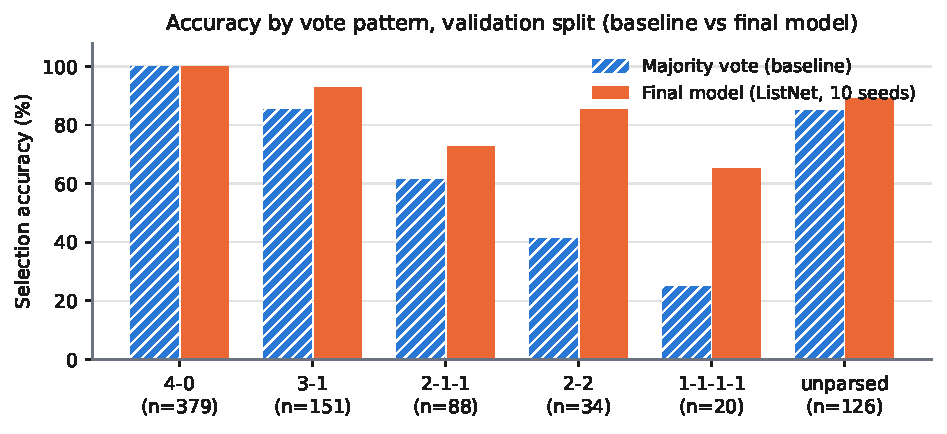
\includegraphics[width=\linewidth]{figures/fig1_patterns.pdf}
\caption{Accuracy by vote pattern on validation. The baseline's deficit is
concentrated in ties and fragmented votes; the learned selector recovers most
of the 2-2 ties (41.2\% $\to$ 85.3\%).}
\label{fig:patterns}
\end{figure}

\section{Method}
\label{sec:method}

\subsection{Group-comparative features}
\label{sec:features}

For every candidate $i$ in group $g$ we compute a $23$-dimensional
handcrafted vector plus the unit-normalised $1024$-dimensional embedding,
$F = 1047$ dimensions in total. All features are functions of the group, never
of the candidate alone (except the style block, which is deliberately
candidate-local and ablated in Section~\ref{sec:ablations}).

\begin{itemize}\itemsep0pt
\item \textbf{Vote agreement (6).} Number of same-answer peers; parseable flag;
group majority size; number of distinct answers; unparsed count; vote margin
against the strongest rival answer.
\item \textbf{Embedding geometry (7).} With $U$ the unit embeddings of the
group and $S = UU^\top$ the $4\times4$ cosine matrix: mean cosine to the other
three candidates; cosine to the group centroid; cosine to the
\emph{majority-answer} centroid (mean of unit embeddings holding a most
frequent answer); mean cosine to same-answer peers and, separately, to
different-answer candidates; a cosine-weighted vote margin
$\sum_{j:\,a_j=a_i} S_{ij} - \sum_{j:\,a_j\neq a_i} S_{ij}$; raw embedding norm.
\item \textbf{Question anchoring (3).} Numeric tokens of the question vs.\ of
the candidate: coverage fraction of question numbers reused, count of missed
question numbers (a candidate that never mentions ``30'' probably ignored the
stop), count of numbers absent from the question.
\item \textbf{Style (7).} Character length (absolute and group-relative), line
count, presence of \verb|\boxed| / \verb|####|, counts of \verb|=| and
\verb|$|. Kept only to test whether the model leans on formatting
(Section~\ref{sec:ablations}).
\end{itemize}

Features are standardised, $z = (f-\mu)/\sigma$, with $\mu,\sigma$ estimated on
the \emph{training} split and stored in the checkpoint; using validation
statistics would leak and destabilise.

\subsection{ListNet group-softmax objective}
\label{sec:listnet}

The metric awards a point for choosing \emph{any} correct candidate, so the
natural target is a distribution over the group rather than a per-candidate
label. With $y_{gi}\in\{0,1\}$ indicating ``candidate $i$'s parsed answer
equals the reference'', define the target distribution
$q_{gi} = y_{gi}/\sum_j y_{gj}$ (uniform over correct candidates), the linear
logits $s_{gi} = w^\top z_{gi} + b$, and the per-group softmax $p_{gi}$.
The loss is the listwise cross-entropy (ListNet top-one probability) plus
weight decay:
\begin{equation}
L = -\frac{1}{N}\sum_{g}\sum_{i} q_{gi}\,\log p_{gi} \;+\; \lambda \lVert w\rVert^2,
\qquad
\frac{\partial L}{\partial s_{gi}} = \frac{p_{gi}-q_{gi}}{N}.
\label{eq:listnet}
\end{equation}
The gradient follows from $\partial \log p_k/\partial s_i = \delta_{ik}-p_i$.
Optimisation: Adam ($\beta_1{=}0.9,\beta_2{=}0.999$), minibatches of 256
\emph{groups}, group order shuffled per epoch with
\texttt{numpy.default\_rng(seed)}, 800 epochs, lr $0.05$, $\lambda{=}3\times10^{-3}$.
Labels come only from the training split references, aligned by \texttt{id}.

Splitting the loss by correctness makes the tie behaviour learnable: on a 2-2
group the target is uniform over the two correct candidates, so the model is
rewarded precisely for the discrimination the baseline gives away.

\subsection{Seed variance and weight averaging}
\label{sec:seeds}

With $1047$ features and $4{,}755$ groups, single-seed validation accuracy
swings between \SEEDMIN\% and \SEEDMAX\% (mean \SEEDMEAN\%). Ensembling is
usually a cost, but for linear scorers the ensemble is free: the mean of $K$
logit functions is itself linear,
$\frac1K\sum_k (z^\top w_k + b_k) = z^\top \bar w + \bar b$,
so averaging the ten weight vectors yields exactly the logit-average model at
\emph{zero} additional assets or latency. This lifts validation to 92.36\% and
is the single cheapest improvement in the project.

\subsection{Inference}
\texttt{predict()} loads \texttt{model.npz} ($w,b,\mu,\sigma$, a
\texttt{with\_emb} flag), builds features with the same function used in
training, standardises, and returns the per-group argmax as a Python
\texttt{int}. With no checkpoint supplied the file degrades to the
deterministic majority vote, so the submission is a legal training-free
baseline on its own.

\section{Experiments}
\label{sec:experiments}

\paragraph{Protocol.} Fitting uses only the 4{,}755 training groups.
Validation guides development and model selection; the test bank was scored
once, after freezing, with the official scorer
(\texttt{predict.py} + \texttt{score\_predictions.py}, fresh processes, four
threads). All ablations below are validation-only by the same discipline.

\subsection{Main result}
The frozen selector scores \textbf{92.36\%} on validation (737/798) and
\textbf{82.66\%} on test (386/467), versus 86.22/69.16 for majority vote:
$+6.1$ points where easy groups still exist and $+13.5$ points on the
all-contested test bank. Per pattern (Table~\ref{tab:patterns},
Figure~\ref{fig:patterns}) the gains concentrate exactly where the analysis
predicted: 2-2 ties $41.2\to85.3\%$, four-way splits $25.0\to65.0\%$, 3-1
$85.4\to92.7\%$. Unanimous groups stay at 100\%: the model never trades the
baseline's free wins for speculative ones.

\subsection{Ablations: which evidence pays?}
\label{sec:ablations}

Each ablation refits the identical pipeline (same hyperparameters, same ten
seeds, same standardisation) on a masked feature subset; validation only.

\begin{table}[t]
\centering\small
\caption{Feature-block ablations, validation accuracy, ten-seed weight average.
Expectations were stated before each run (right column).}
\label{tab:ablations}
\begin{tabular}{lrlp{6.4cm}}
\hline
Variant & $F$ & Val\,\% & Stated expectation \\
\hline
hand only (no embeddings) & 23 & \ABHAND & close to baseline: votes alone cannot read the traces \\
embeddings only (no hand) & 1024 & \ABEMB & clearly above chance but below full: semantics without comparison cues \\
full $-$ style & 1040 & \ABNOSTYLE & $\approx$ full: style should carry (almost) nothing \\
full $-$ anchoring & 1044 & \ABNOANCHOR & slightly below full: dropped-condition signal is real but small \\
\textbf{full} & 1047 & \textbf{92.36} & -- \\
\hline
\end{tabular}
\end{table}

\paragraph{Does reading the reasoning help?} Yes, through two complementary
channels. Hand features alone (votes, geometry, style, anchoring -- no trace
embeddings) sit at \ABHAND\%, $+2.9$\,pp over the 86.2\% baseline: knowing
\emph{how many} candidates agree, and how their traces sit geometrically, adds
modestly to counting votes. Embeddings alone, with no cross-candidate feature
except the raw unit trace vectors, reach \ABEMB\% ($+3.7$\,pp): the frozen
trace embedding already carries semantic evidence about which derivation is
sound, even without being told what its siblings said. Combining both gives
92.36\% ($+3.3$ over hand-only, $+2.4$ over embeddings-only): reading the
reasoning -- directly through the embedding, and comparatively through the
group features -- is where the accuracy comes from.

\paragraph{Is it a style shortcut?} No. Removing all seven length/format
features costs nothing at all (\ABNOSTYLE\%, identical to the full model to
four decimals). Independently, the learned weights
confirm it (Table~\ref{tab:weights}): the $\ell_2$ norm of the style block is
$0.059$ against $0.841$ (vote), $0.324$ (anchoring) and $0.289$ (geometry); the
largest single handcrafted weight is the \emph{parseable} flag ($+0.84$), i.e.\
``an unparseable final answer is rarely a correct one'', which is a correctness
cue, not a formatting cue. The GUIDE's worry -- winning by sounding confident --
is not how this model wins.

\begin{table}[t]
\centering\small
\caption{Largest handcrafted weights of the frozen bundle (features are
standardised with train-split statistics, so weights are directly comparable),
and block/family norms. Reproduced by \texttt{analyze.py}.}
\label{tab:weights}
\begin{tabular}{rlrl}
\hline
\# & feature & weight & family \\
\hline
1 & parseable & $+0.839$ & vote \\
2 & numbers not in question & $+0.303$ & anchor \\
3 & cos to same-answer peers & $-0.222$ & geometry \\
4 & cos to majority centroid & $+0.161$ & geometry \\
5 & question-number coverage & $+0.101$ & anchor \\
6 & cos to different-answer & $+0.075$ & geometry \\
7 & vote margin & $+0.053$ & vote \\
8 & missed question numbers & $-0.050$ & anchor \\
\hline
\multicolumn{4}{l}{family norms: vote $0.841$, anchor $0.324$, geometry $0.289$, style $0.059$} \\
\multicolumn{4}{l}{block norms: $\lVert w_{\text{emb}}\rVert = 1.815$, $\lVert w_{\text{hand}}\rVert = 0.948$} \\
\hline
\end{tabular}
\end{table}

\paragraph{Should a solution be judged on its own?} No. The embeddings-only
variant judges each candidate from its own trace vector (plus whatever the
linear layer can extract from it), and lands at \ABEMB\%; adding the explicit
group-comparative structure (vote margins, cosine-to-majority, cosine-weighted
margin) closes the remaining $+2.4$\,pp. A candidate that looks plausible in
isolation is exposed by its siblings: the largest gains sit exactly in the
tie patterns where isolation gives the baseline no information at all
(2-2: $41.2\to85.3\%$, Figure~\ref{fig:patterns}). Comparison, not isolated
plausibility, is the operative signal.

\subsection{Seed variance and rejected variants}
Single seeds span \SEEDMIN--\SEEDMAX\% (mean \SEEDMEAN\%, Table~\ref{tab:seeds});
the ten-seed weight average (92.36\%) sits above the single-seed mean and
removes the luck factor from model selection. Note that the averaged model
matches the best single seed (seed~0, 92.36\%) here by a coincidence of this
bank; on the development runs the average was chosen precisely because single
seeds move by $\pm1.3$\,pp. Three more elaborate ideas were tried and rejected,
and we report them because they are informative:

\begin{table}[t]
\centering\small
\caption{Single-seed validation accuracy of the final feature set (seeds 0--9),
and the ten-seed weight average. Reproduced by \texttt{seed\_sweep.py};
raw values in \texttt{runs/analysis/seeds.json}.}
\label{tab:seeds}
\begin{tabular}{lcccccccccc|c}
\hline
seed & 0 & 1 & 2 & 3 & 4 & 5 & 6 & 7 & 8 & 9 & mean \\
\hline
val\,\% & 92.36 & 89.72 & 91.10 & 91.85 & 90.85 & 90.98 & 90.48 & 89.97 & 91.48 & 90.98 & 90.98 \\
\hline
\end{tabular}

\vspace{0.5em}
ten-seed weight-averaged model: \textbf{92.36\%}
\end{table}
\begin{itemize}\itemsep0pt
\item \textbf{MLP} (128-unit hidden layer, same features): 91.4--92.4\% per
seed, ensemble 92.36\% -- no gain over linear at $>100\times$ the parameters.
The signal in these features is essentially linearly separable.
\item \textbf{Deviation embeddings} ($u_i - \bar u_g$, 1024 extra dims):
87--89\%, i.e.\ \emph{worse} than the plain embedding variant; the deviation
block overfits group noise.
\item \textbf{Group weighting} (down-weighting all-correct groups in the loss):
91.7--92.0\%, no gain; the uniform-over-correct target already handles them.
\end{itemize}

\subsection{Resources}
Training (ten seeds, 800 epochs, CPU NumPy) takes $\approx192$\,s on the
development machine (AMD Ryzen 7 9800X3D, 8 cores). Official evaluation of the
complete test bank -- one fresh prediction process plus one fresh scoring
process, four threads across libraries -- takes $0.21 + 0.11 \approx 0.32$\,s
here, against a 30\,s budget on the reference Xeon Platinum 8457C. The entire
inference asset is \texttt{model.npz} at $26{,}347$ bytes (limit 16\,MiB).
More computation (MLP, deviation embeddings) bought nothing; the cheap linear
model is also the accurate one. Table~\ref{tab:resources} states the budgets
and the measurements side by side.

\begin{table}[t]
\centering\small
\caption{Resource use against the assignment limits. Local: AMD Ryzen 7
9800X3D, 8 cores; reference: Xeon Platinum 8457C, 4 threads total.}
\label{tab:resources}
\begin{tabular}{lll}
\hline
Quantity & Limit & Measured (local) \\
\hline
Inference wall time, fresh predict+score processes & 30\,s (reference CPU) & 0.32\,s \\
Inference assets (weights, statistics, config) & 16\,MiB & 26{,}347\,B \\
Training hardware & CPU or $\le$ RTX 4090 & CPU only \\
Training cost, one 10-seed bundle & -- & $\approx$192\,s \\
Inference dependencies & -- & Python 3.13.9, NumPy 2.5.4 \\
\hline
\end{tabular}
\end{table}

\section{Analysis: confidence, and where the model still fails}
\label{sec:analysis}

\subsection{The model cannot read its own uncertainty}
A natural question from the brief is whether high scores track correct
choices. For this model, \emph{no} -- and the negative result is cleaner than
any hedge. On contested validation groups, bucketing by the logit margin
(top1 $-$ top2) gives accuracies 84.5 / 80.3 / 81.7 / 83.1 / 84.5\% across
margin quintiles (Figure~\ref{fig:calibration}): flat. The rank correlation
style statistic $P(\text{margin}_{\text{correct}} > \text{margin}_{\text{wrong}})$
is $0.520$ on contested groups -- chance is $0.5$. Absolute softmax
probabilities are worse than flat: the expected calibration error over seven
bins is $0.52$, because the group softmax is a \emph{ranking} loss and its
outputs are not probability estimates (mean $p_{\text{top}} \approx 0.40$ at
92\% accuracy: grossly underconfident).

\begin{figure}[t]
\centering
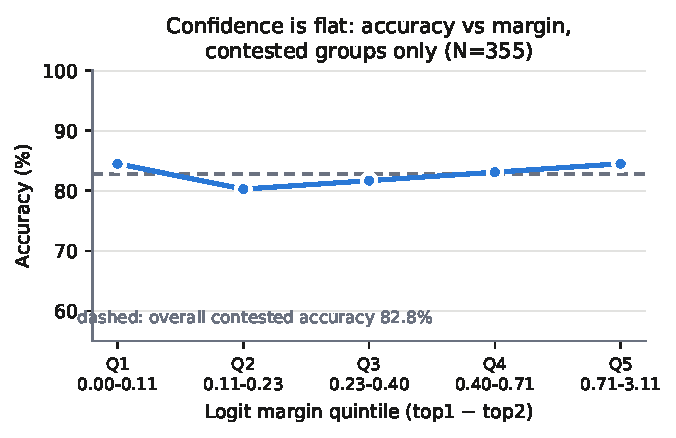
\includegraphics[width=0.72\linewidth]{figures/fig2_calibration.pdf}
\caption{Accuracy versus logit-margin quintile on the 355 contested validation
groups. The curve is flat around the 82.8\% contested mean: the model's
confidence does not rank its own correctness.}
\label{fig:calibration}
\end{figure}

Two readings. (i) On unanimous groups the margin is near zero \emph{by
construction} (four nearly identical feature rows) yet accuracy is 100\%, so
any global confidence measure is confounded by vote pattern; the honest
calibration question must be asked within contested groups, where the answer is
flat (Table~\ref{tab:calibration}). (ii) A listwise loss trained to separate
correct from incorrect \emph{within} a group has no incentive to make margins
comparable \emph{across} groups. Making confidence meaningful would need an
explicit calibration or abstention objective -- out of scope here, since the
task forces a choice on every question. We report this as the main limitation:
the selector is accurate but not self-aware.

\begin{table}[t]
\centering\small
\caption{Accuracy by logit-margin quintile on the 355 contested validation
groups (each quintile $N=71$). The relation is flat around the 82.8\%
contested mean; separation $P(\text{margin}_{\text{correct}} >
\text{margin}_{\text{wrong}}) = 0.520$.}
\label{tab:calibration}
\begin{tabular}{lccccc}
\hline
margin quintile & Q1 & Q2 & Q3 & Q4 & Q5 \\
range & 0.00--0.11 & 0.11--0.23 & 0.23--0.40 & 0.40--0.71 & 0.71--3.11 \\
acc\,\% & 84.5 & 80.3 & 81.7 & 83.1 & 84.5 \\
\hline
\end{tabular}
\end{table}

\subsection{Residual errors}
The 61 validation errors sit in 2-1-1 (24), 3-1 (11), unparsed groups (14),
2-2 (5) and four-way splits (7). The dominant failure is the ``confident
minority-wrong / majority-wrong'' case: when two or three candidates share a
misreading of the question (the bus-stop pattern of the brief: dropping one
condition), their traces cluster tightly and their votes reinforce each other,
and the geometry features that usually expose a lone deviator instead support
the wrong consensus. Inspecting weights is consistent: cosine to same-answer
peers carries a \emph{negative} weight ($-0.22$) once vote counts are
conditioned on -- tight same-answer clusters are, counter-intuitively, mild
evidence of shared error -- while cosine to the majority centroid is positive
($+0.16$). The two partially cancel, which is likely why the four-way and
2-1-1 patterns improve least.

\subsection{A failure case study: double counting}
\label{sec:case}
Validation question \texttt{gsm8k:47ea45\ldots}: ``Texas Integrated School has
15 classes and has 20 students per class. They added five more classes, how
many students will they have now?'' (reference: $400$). All four candidates
agree on every intermediate quantity -- $15\times20=300$, $15+5=20$ classes,
$20\times20=400$ -- and split 2--2 only on the final step: the correct pair
\emph{replaces} the old total with the new one ($400$), while the wrong pair
\emph{adds} the new total on top of the old one ($300+400=700$), counting the
same 400 students twice.

The model ranks the wrong cluster first (logits $+1.74,+1.01$ for the 700 pair
vs.\ $+0.93,+0.63$ for the 400 pair), and no feature it is allowed to use can
see why: the numeric-coverage features are identical across all four traces
(every question number appears in every candidate), the vote is a tie, the
embedding geometry is nearly symmetric because the four traces differ only in
one closing addition, and the frozen whole-trace embedding averages that single
step away together with the rest of the derivation. This is the sharpest form
of the limitation above: the available evidence is \emph{invariant} to the
distinction that decides the question. Step-level features, or a verifier that
re-executes each arithmetic line, would be needed; both exceed the asset and
runtime budget this project set itself.

\section{Reproducibility}
\label{sec:repro}

\paragraph{Environment.} Python 3.13.9, NumPy 2.5.4 (Matplotlib only for
report figures), Windows 11, AMD Ryzen 7 9800X3D; no GPU, no external weights
or data. Protocol string: \texttt{dase7506-mp2-open-hard-verifier-v5}.

\paragraph{Commands.} From \texttt{code/}:
\begin{verbatim}
python check_data.py
python train.py --variant emb --seeds 10 \
    --out runs/model_bundle
OMP_NUM_THREADS=4 OPENBLAS_NUM_THREADS=4 \
MKL_NUM_THREADS=4 python predict.py \
    --method submission.py \
    --checkpoint runs/model_bundle \
    --split test \
    --output runs/test-predictions.json
python score_predictions.py --split test \
    --predictions runs/test-predictions.json \
    --output runs/test-score.json
\end{verbatim}
Analysis and figures: \texttt{python analyze.py}, \texttt{python ablations.py},
\texttt{python make\_figures.py}. Seeds $0\dots9$ for the submitted model;
every random source goes through \texttt{default\_rng}.

\paragraph{Artefacts and checks.}
Official scores: validation $92.35588972431077$ (737/798), test
$82.65524625267666$ (386/467); JSONs in \texttt{runs/}. Asset SHA-256:
\texttt{e0181539\ldots a1cbcde} (\texttt{runs/model\_bundle/model.npz},
26{,}347\,B); hyperparameters and byte count recorded in
\texttt{meta.json}. Determinism: a full retrain reproduces the bundle
bit-identically (identical SHA-256) and the same scores. Audit robustness:
\texttt{predict()} was called on a randomly drawn, shuffled 37-question
sub-bank of validation; it returns valid ints and its choices agree exactly
with the full-bank run (features are per-group by construction, so no
order or size dependence exists). Test references were used only for the two
official scoring runs above.

\section{Limitations and conclusion}
The scorer rewards only the final number, so the method optimises
answer-plausibility, not reasoning validity; a candidate with a broken
intermediate step and a lucky final number is indistinguishable from a clean
one by design of the metric. The embeddings are frozen, so no new
representations could be learned, and the linear form -- validated by the MLP
ablation -- caps expressiveness at what these features already separate.
Confidence is unusable for abstention or routing (Section~\ref{sec:analysis}).
Within those limits, group-comparative linear scoring turns a 69.2\% test
baseline into 82.7\% with a 26\,KB asset and a third of a second, and the
ablations locate the gain precisely: cross-candidate comparison and trace
semantics, not formatting.

\section*{AI assistance and reuse disclosure}
The methodological ideas -- the group-comparative feature design, the ListNet
formulation, the seed-weight-averaging trick and the experiment plan -- were
developed in discussion with an AI assistant (Claude, Anthropic); the author
implemented, reproduced and verified all code after understanding it, ran every
experiment reported here, and takes full responsibility for the submitted
implementation and numbers. No external code, datasets or pretrained weights
were used beyond the supplied package; GSM8K and Qwen3-0.6B attributions are
kept as supplied.

\begin{thebibliography}{9}\small
\bibitem{gsm8k} Cobbe et al., \emph{Training Verifiers to Solve Math Word
Problems} (GSM8K), 2021.
\bibitem{listnet} Cao et al., \emph{Learning to Rank: From Pairwise Approach
to Listwise Approach}, ICML 2007.
\bibitem{qwen3} Qwen Team, \emph{Qwen3 Technical Report}, 2025 (candidate
generator only; no weights distributed here).
\end{thebibliography}

\end{document}
